\begin{thm}[The Pigeonhole Principle]\index{pigeonhole principle}
    Given finite sets \(X\) and \(Y\) with \(|X|>|Y|\), a function from \(f:X\longrightarrow Y\) can not be one-to-one.  Moreover, if \(k<|X|/|Y|\), then there exists some \(y\in Y\) such that \(|f^{-1}(y)|\geq k+1\).\vspace{\baselineskip}

    For example given \(X=\left\{1,\ldots,11\right\}\) and \(Y=\left\{1,\ldots,4\right\}\), \(|X|=11>|Y|=4\) and \(11/4>2\); for any function there will be some \(y\) such that \(|f^{-1}(y)|\geq 2+1=3\).
    \begin{figure}[H]
        \centering
        % \inputtikz{sample_pigeons}
        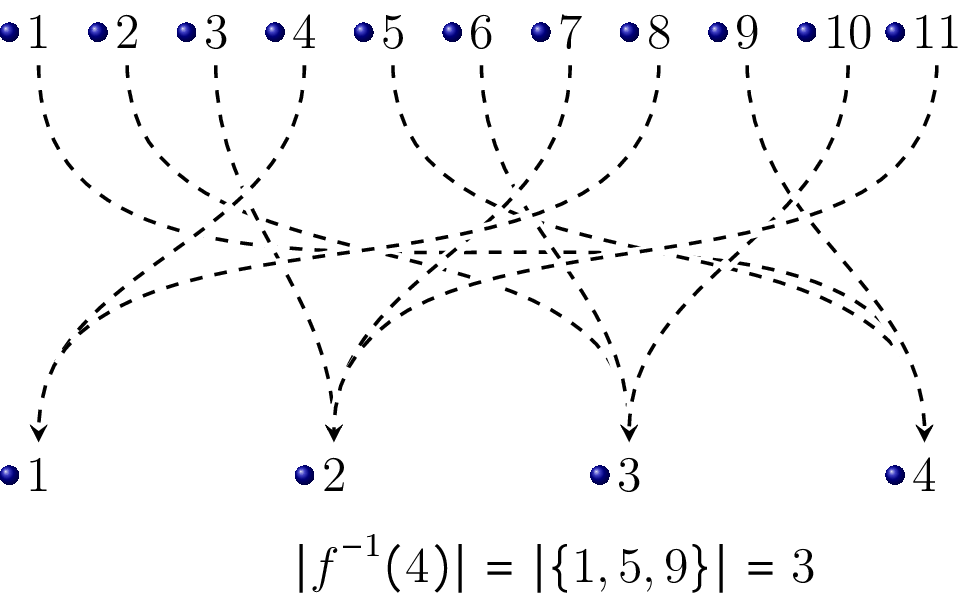
\includegraphics[scale=0.24,alt={illustration of the pigeonhole principle}]{images/created/sample_pigeons.png}
        \caption{Pigeonhole Demonstration}
        \label{fig:pigeon}
    \end{figure}
\end{thm}

\begin{practiceprob}
    If the Citadel in Old Town sends out 21 ravens to 12 castles around Westeros announcing that ``\textfrak{Winter is Coming!!!}'' why is there at least one castle that receives 2 ravens?
    \begin{figure}[H]
        \centering
        % \inputtikz{westros}
        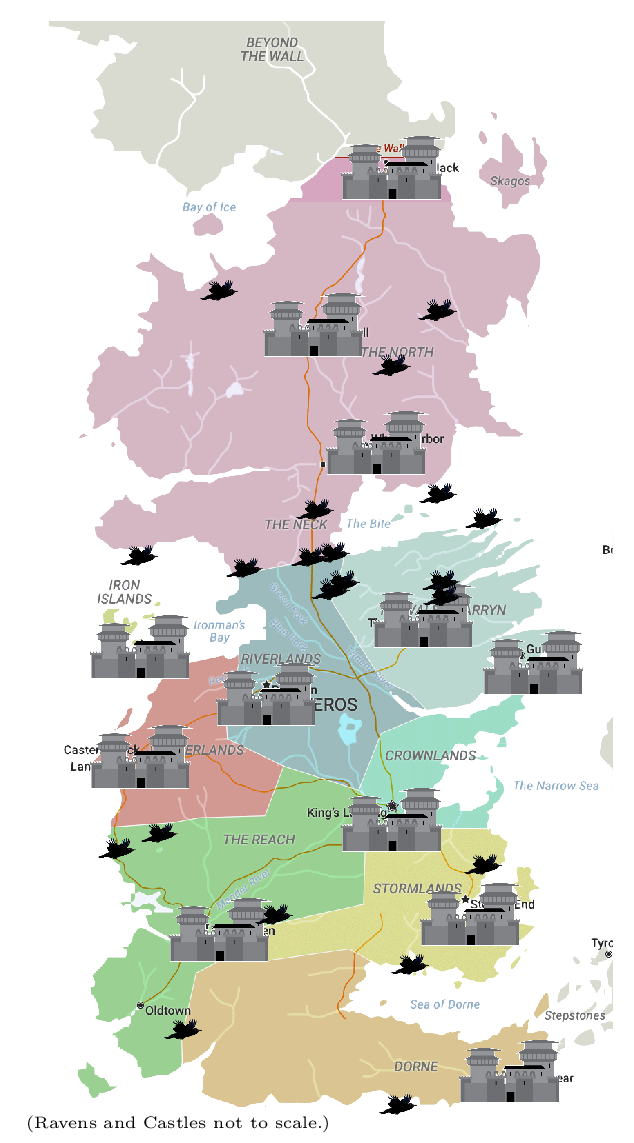
\includegraphics[scale=0.2,alt={ravens flying over westros}]{images/created/westros.png}
        \caption{Westros}
        \label{fig:westros}
    \end{figure}
\end{practiceprob}

\clearpage

\begin{practice}{Pigeonhole Principle: Picking Things Out}
    Given the set of integers \(X=\{1,...,9\}\) any set of six numbers selected at random will have at least two which sum to 10.
        % \[S_1=\{1,9\}, S_2=\{2,8\}, S_3=\{3,7\}, S_4=\{4,6\}, S_5=\{5\}\]
    \vspace{0.2\textheight}
\end{practice}

\begin{practice}{Pigeonhole Principle: Remainders}
    If an integer \(n\) is divided by 7, and \(n\) is not a multiple of 7, then the number of repeating digits is at most 6. (Try \(37\div 7\).)
    \vspace{0.2\textheight}
\end{practice}

\begin{practice}{Generalized Pigeonhole Principle: Sharing Tables}
    Given 10 lunch tables and 57 students, show that there must be at least one table with six students.
    \vspace{0.2\textheight}
\end{practice}

\begin{thm}
    Given finite sets \(X\) and \(Y\), there exists a one-to-one and onto function from \(X\) to \(Y\) if and only if \(|X|=|Y|\).
\end{thm}